\cleardoublepage

\section{引言}

\subsection{研究背景}
近年来,神经网络的成功应用促进了模式识别和数据挖掘等领域的研究。许多机器学习任务
,如目标检测[1],机器翻译[2]和语音识别[3],曾经非常依赖人工来提取特征信息,现在可
以通过各种端到端深度学习范式来完成,如卷积神经网络[4],循环神经网络[5]和自动编码
器[6]。深度学习在很多领域的成功归功于快速发展的计算资源(GPU)、大量可用于训练的
数据、以及从欧几里得数据(图像、文本、视频)中提取特征的能力。以图像数据为例,我们
可以将欧几里得空间中的图像表示为规则网络,卷积神经网络能够利用图像数据的平移不变性、
局部连通性和合成性来提取特征,因此卷积神经网络可以提取能够应用于整个数据集的局部有效
特征信息。

虽然深度学习可以有效地捕捉欧几里得数据的特征,但越来越多的应用程序将数据表示为图数据。
人们处理和分析非结构化的数据的需求正在日益增长,如社交网络[7]、交通网络[8]、推荐系
统[9]、组合优化问题中[10]的数据,这些数据之间的关系是复杂的,对应于一个已知或未知的
图结构。具体来说,在电子商务中,推荐系统需要利用用户浏览过的产品,为用户推荐新产品,这些产
品之间的联系就是图结构的;在药物研发领域[11],每个药物分子可以表示为各种化学结构的图结构,为
了加快药物的研发速度,需要用利用分子的潜在表征来估计化学性质,这涉及到图上的编码和解
码过程;在芯片设计过程中[12],标准晶片单元的放置和路线会影响晶片的功率、晶片模具尺寸
和性能,所以芯片图上单元摆放和连接的设计任务,需要处理图结构和图数据。与网格数据相比,
图数据无疑是一种更加通用、应用更广的数据。

然而,图数据的复杂性给现有的机器学习算法带来了巨大的挑战,这主要有以下两个原因。首先,
图是不规则的,图上的节点是无序的且可变的,每个节点可能有不同数量的邻居,这导致一些重要
的操作(如卷积运算)很容易在图像域计算,但很难应用到图域;此外,现有机器学习算法的一个核
心假设是实例之间是相互独立的,但这个假设不再适用于图数据,因为每个实例都通过潜在的图结构与其他实例相关联。

\subsection{研究现状}
为了处理和利用图数据,在图信号处理领域,有学者提出了图信号的高效表示方法,并且建立
了关于图的移位、滤波、卷积、傅立叶变换、频谱分解等一系列概念[13,14,15];此外,有
很多研究者尝试使用图变换算子(GSO)的矩阵多项式[16],来设计可以分析图信号和设计的图
滤波器,这些图滤波器可以被用于信号预测、信号压缩、分类任务等应用。

在深度学习领域,也正在有越来越多关于图神经网络(GNNs)的研究。学者们先
后提出了递归图神经网络(RecGNNs)、图卷积神经网络(ConvGNNs)、图自编码器
(GAEs)、时空图神经网络(STGNNs)等神经网络结构,见图\ref{1-1}。其中,ConvGNNs 汲取了图信
号处理领域的思想,将卷积运算从网格数据推广到图数据。目前,ConvGNNs 已经
在节点级分类的半监督学习、图级分类的监督学习、用于图嵌入的无监督学习等任务里取得
了前所未有的效果;并且在其他复杂的GNNs 模型中,ConvGNNs 也发挥着核心作
用。

\begin{figure}[htbp]
    \centering
    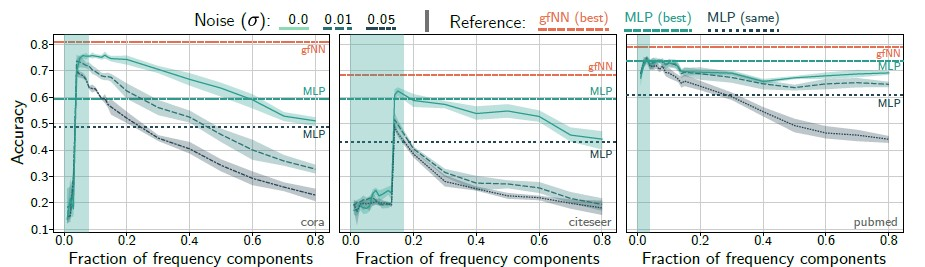
\includegraphics[width=12cm]{introduction/1.jpg}
    \caption{\label{1-1}图神经网络(GNNs)的分类}
\end{figure}

\subsubsection{递归图神经网络(RecGNNs)}
RecGNNs大多是图神经网络的先驱作品。RecGNNs的目的是通过循环神经网络结构,来学习节点
表示。他们假设图中的一个节点不断地与它的邻居交换信息,直到达到一个稳定的均衡。
RecGNNs在概念上很重要,启发了图卷积神经网络的后续研究,特别是,基于空间的图卷积神经
网络继承了信息传递的思想[17]。

\subsubsection{图卷积神经网络(ConvGNNs)}
ConvGNNs将卷积运算从网格数据推广到图数据。其主要思想是通过聚合节点$v$自身的特征$x_{v}$
和邻居的特征$x_{u}$来生成节点$v$的表示,其中$u\in N(v)$。与RecGNNs不同,ConvGNNs将多个
图卷积层堆叠起来,提取高级节点表示。在建立许多其他复杂的GNN模型中,ConvGNNs发挥着核心作
用。如图\ref{1-2}中ConvGNN被用于节点的分类,图\ref{1-3}中ConvGNN被用于图的分类。
\begin{figure}[htbp]
    \centering
    \captionsetup{width=10cm}
    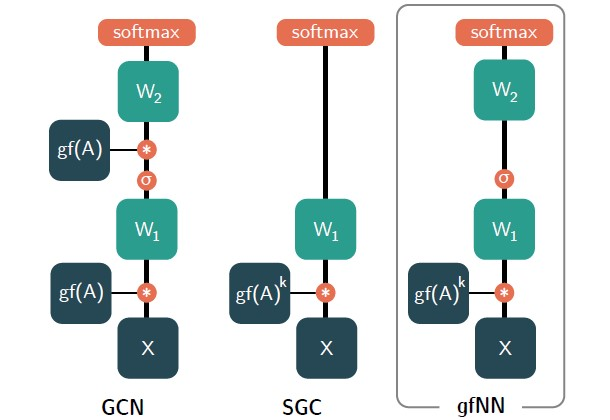
\includegraphics[width=12cm]{introduction/2.jpg}
    \caption{\label{1-2}通过堆叠多层卷积层,来获得邻节点的信息,用于节点的分类。}
\end{figure}

\subsubsection{图自编码器(GAEs)}
GAEs是一种无监督学习框架,它将节点或图编码成一个潜在的向量空间,并从编码的信息重构图数据。
该算法用于学习网络嵌入和图生成分布。对于网络嵌入,GAEs通过重构图的邻接矩阵等图结构信息来
学习潜在节点表示[18],如图\ref{1-4}。对于图的生成,有的方法是一步一步生成图的节点和边,有的
方法是一次性输出图。
\begin{figure}[htbp]
    \centering
    \captionsetup{width=10cm}
    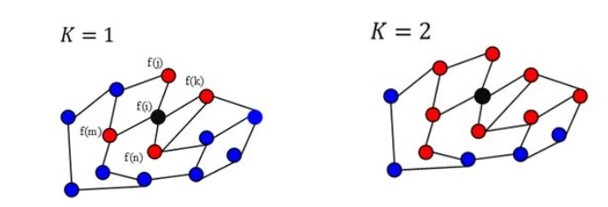
\includegraphics[width=12cm]{introduction/3.jpg}
    \caption{\label{1-3}通过卷积层和池化层,来提取特征信息,并最终用于图的分类。}
\end{figure}
\begin{figure}[htbp]
    \centering
    \captionsetup{width=10cm}
    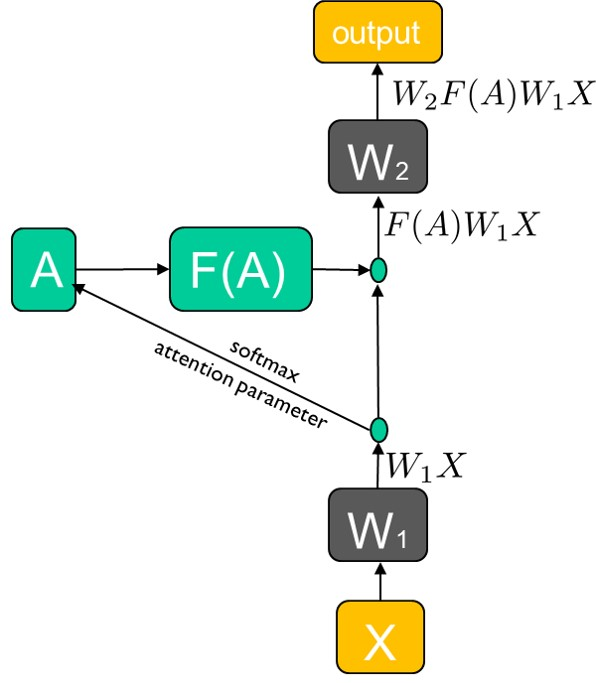
\includegraphics[width=12cm]{introduction/4.jpg}
    \caption{\label{1-4}编码器使用图卷积层得到每个节点的网络嵌入,解码器重构图邻接矩阵。}
\end{figure}

\subsubsection{时空图神经网络(STGNNs)}
STGNNs的目的是从时空图中学习隐藏的模式,这在各种应用中变得越来越重要,如交通速度预测,驾驶员操纵
预测,人类行为识别。STGNNs的核心思想是同时考虑空间依赖和时间依赖。目前的许多方法都是通过图卷
积来捕获与RNNs或CNNs的空间依赖关系,从而对时间依赖关系进行建模,如图\ref{1-5}。
\begin{figure}[htbp]
    \centering
    \captionsetup{width=10cm}
    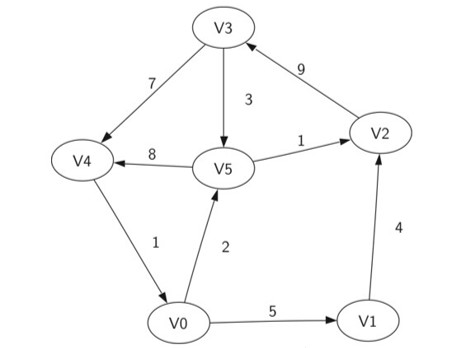
\includegraphics[width=12cm]{introduction/5.jpg}
    \caption{\label{1-5}图卷积层对$A$和$X^(t)$进行操作以捕获空间特性,而1D-CNN层沿时间轴在$X$上滑动以捕获时间特性。}
\end{figure}

% \begin{figure}[htbp]
%     \centering
%     \begin{minipage}[t]{0.48\textwidth}
%     \centering
%     \captionsetup{width=6cm}
%     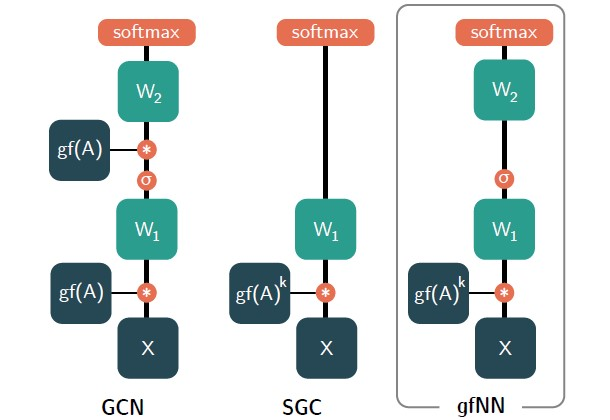
\includegraphics[width=8cm]{introduction/2.jpg}
%     \caption{\label{1-2}通过堆叠多层卷积层,来获得邻节点的信息,用于节点的分类}
%     \end{minipage}
%     \begin{minipage}[t]{0.48\textwidth}
%     \centering
%     \captionsetup{width=6cm}
%     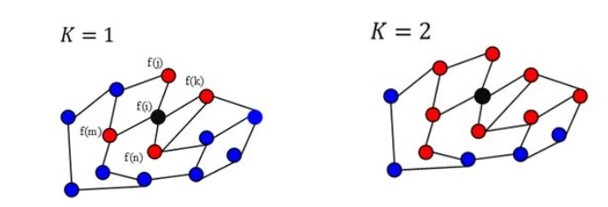
\includegraphics[width=8cm]{introduction/3.jpg}
%     \caption{\label{1-3}通过卷积层和池化层,来提取特征信息,并最终用于图的分类}
%     \end{minipage}
% \end{figure}
% \begin{figure}[htbp]
%     \centering
%     \begin{minipage}[t]{0.48\textwidth}
%     \centering
%     \captionsetup{width=6cm}
%     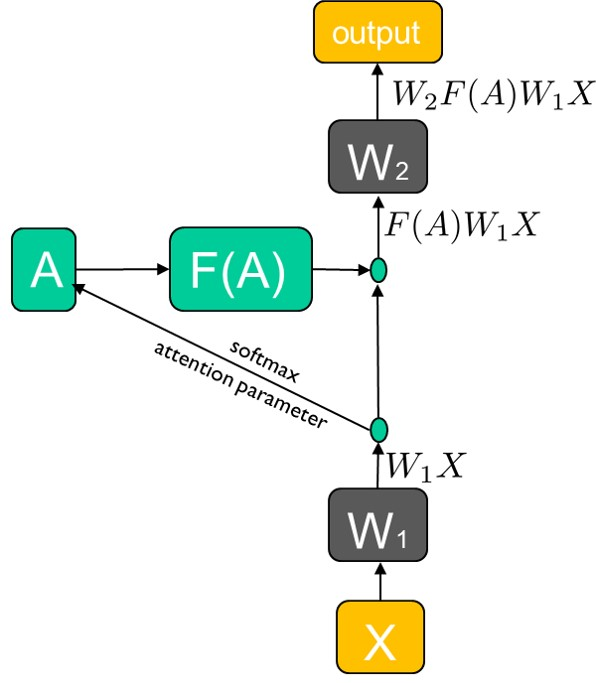
\includegraphics[width=8cm]{introduction/4.jpg}
%     \caption{\label{1-4}编码器使用图卷积层得到每个节点的网络嵌入,解码器重构图邻接矩阵}
%     \end{minipage}
%     \begin{minipage}[t]{0.48\textwidth}
%     \centering
%     \captionsetup{width=6cm}
%     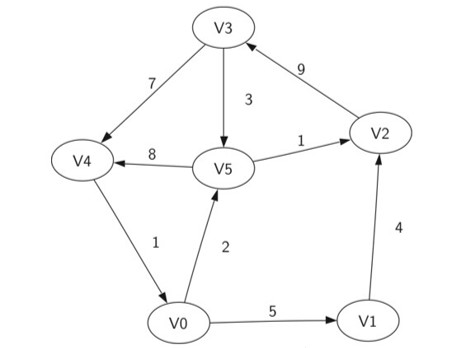
\includegraphics[width=8cm]{introduction/5.jpg}
%     \caption{\label{1-5}图卷积层对$A$和$X^(t)$进行操作以捕获空间特性,而1D-CNN层沿时间轴在$X$上滑动以捕获时间特性}
%     \end{minipage}
% \end{figure}

\subsection{主要贡献}
我们工作的主要贡献总结如下:
\begin{itemize}
    \item \textbf{设计新的图卷积神经网络} \quad
    我们从“图卷积神经网络能够等效于低通滤波器”这一结论出发,将频谱理论和空间理论的设计方法相结合,设计
    了一种具有高效率和强表达能力的新图卷积神经网络(poly GAT),并且在Cora和Citeseer数据集上
    测试了我们新神经网络的性能。
    
    \item \textbf{提供设计的新思路} \quad
    我们创新性地提出,将频谱理论中的矩阵多项式表示方法,和空间理论中的注意力机制表示方法相结合的图卷积网络
    设计方法。图注意力机制能够灵活地学习节点之间的关系,我们的设计重点是如何更充分地利用注意力矩阵中蕴含的信
    息。这样的设计思路,是十分新颖的,我们设计的网络poly GAT也验证了这一思路的可行性。
\end{itemize}

\subsection{论文结构}
这篇毕业论文的行文结构如下。第2节,做为图卷神经网络设计的理论基础,我们分别介绍了基于频谱理论和基于空间理论
的设计方法,并且分析了它们的区别和优劣;第3节,我们从图信号处理领域的结论出发,阐述了我们的设计思路,并且详
述了我们所提出的新图卷积神经网络(poly GAT)的结构;第4节,我们在Cora等数据集上测试了我们的新网络,
并且做了一系列相关实验,验证了其高效率和强大的表达能力;第5节,我们讨论和展望未来潜在的研究方向。